\documentclass[10pt]{beamer}

% mac版,texShop 中Typeset选择 XeLaTex 

%%%%%%%%%%%%%%%%%%%%%%%%%%%%%%%%%%%%%
\usepackage[slantfont,boldfont]{xeCJK}
%\input{xecjkfonts},CJKtextspaces
\setCJKmainfont{STKaiti}   % STFangsong 设置缺省中文字体
\setCJKmonofont{SimSun}   % 设置等宽字体
\setmainfont{Times} % 英文衬线字体
\setmonofont{Times} % 英文等宽字体
\setsansfont{Times} % 英文无衬线字体
%%%%%%%%%%%%%%%%%%%%%%%%%%%%%%%%%%%%%%

\mode<presentation> {
  %\usetheme{Madrid}
  %\usetheme{Singapore}
  \usetheme{Warsaw}
  \setbeamercovered{transparent}
 % \usefonttheme[onlymath]{serif}  
 \usefonttheme{professionalfonts}%{structurebold}
 % \usefonttheme[onlymath]{structurebold}
  \usecolortheme{rose}
}

\usepackage[english]{babel}
%\usepackage[latin1]{inputenc}

%\usepackage{times}
%\usepackage[T1]{fontenc}


%\usepackage{epsfig}
\usepackage{graphics}
\usepackage{color}
\usepackage{amsmath,amssymb,mathrsfs}
\usepackage{amsfonts,stmaryrd}
%\usepackage{thmmarks}
%\usepackage{}



\newcommand\frakfamily{\usefont{U}{yfrak}{m}{n}}
\DeclareTextFontCommand{\textfrak}{\frakfamily}
\def\diag{\mathrm{diag}}


\title[数值计算方法]{数值计算方法}
\subtitle{-对称正定矩阵的分解及迭代法求解线性方程组}


\subject{Talks}

% If you have a file called "university-logo-filename.xxx", where xxx
% is a graphic format that can be processed by latex or pdflatex,
% resp., then you can add a logo as follows:

% \pgfdeclareimage[height=0.5cm]{university-logo}{university-logo-filename}
% \logo{\pgfuseimage{university-logo}}

%\pgfdeclareimage[height=0.5cm]{university-logo}{ncsu_logo}
%\logo{\pgfuseimage{university-logo}}

% Delete this, if you do not want the table of contents to pop up at
% the beginning of each subsection:
%\AtBeginSubsection[] {
%  \begin{frame}<beamer>
%    \frametitle{Outline}
%    \tableofcontents[currentsection,currentsubsection]
%  \end{frame}
%}

% If you wish to uncover everything in a step-wise fashion, uncomment
% the following command:

% \beamerdefaultoverlayspecification{<+->}


\setbeamertemplate{theorems}[numbered]
\setbeamertemplate{caption}[numbered]


\newtheorem{proposition}[theorem]{Proposition}

%%%%%%%%%%%%%%%%%%%%%%%%%%%
% REMARK-STYLE-ENVIRONMENTS %
%%%%%%%%%%%%%%%%%%%%%%%%%%%
\newcounter{remark}
% \numberwithin{theorem}{section}
\def\openrem#1#2{\refstepcounter{remark}\bigskip

{\noindent\bf#1~\theremark\if#2!{. }\else{ (#2).}\fi}
\it}
\def\thmskip{}
\newenvironment{remark}[1][!]{\openrem{Remark}{#1}}{\thmskip}

%%%%%%%%%%%%%%%%%%%%%%%%%%%%
%% AlGORITHM-STYLE-ENVIRONMENTS %
%%%%%%%%%%%%%%%%%%%%%%%%%%%%
\newcounter{algorithm}
% \numberwithin{theorem}{section}
\def\openalg#1#2{\refstepcounter{algorithm}\bigskip

{\noindent\bf#1~\thealgorithm\if#2!{. }\else{ (#2).}\fi}
\it}
\def\thmskip{}
\newenvironment{algorithm}[1][!]{\openrem{Algorithm}{#1}}{\thmskip}
%
%
%%%%%%%%%%%%%%%%%%%%%%%%%%%%
%% Result-STYLE-ENVIRONMENTS %
%%%%%%%%%%%%%%%%%%%%%%%%%%%%
%\newcounter{result}
%\def\openrem#1#2{\refstepcounter{result}\bigskip
%{\noindent \it \bfseries#1~\theremark\if#2!{. }\else{ (#2). }\fi}}
%\newenvironment{result}[1][!]{\openrem{Result}{#1}}{\qed}




%%%%%%%%%%%%%%%%%%%%%%%%%%%
%Redefine the Symbols%
%%%%%%%%%%%%%%%%%%%%%%%%%%%

\def\mathbi#1{\textbf{\em #1}}

% integrals
\def\dx{\,{\rm d}x}
\def\dxb{\,{\rm d}\boldsymbol{x}}
\def\dy{\,{\rm d}y}
\def\dt{\,{\rm d}t}
\def\ds{\,{\rm d}s}
\def\du{\,{\rm d}u}

\def\dr{\,{\rm d}r}
\def\dtheta{\,{\rm d}\theta}

\def\dd{{\rm d}}

\def\intOm{\int_{\Omega}}
\def\intbOm{\int_{\partial \Omega}}

% differences
\def\Dx{\Delta x}
\def\Dt{\Delta t}
\def\D{\Delta}


% operators
\def\Ls{\mathscr{L}}

% matirices
\def\Js{\mathscr{J}}


%fields%
\def\R{\mathbb{R}}
\def\N{\mathbb{N}}
\def\Z{\mathbb{Z}}

%Spaces%
\def\H{\mathbb{H}}
\def\L{\mathbb{L}}
\def\P{\mathbb{P}}


\def\U{\mathbb{U}}
\def\V{\mathbb{V}}
\def\W{\mathbb{W}}
\def\X{\mathbb{X}}
\def\Y{\mathbb{Y}}

\def\Cinfty{C^\infty}




%vectors%
\def\ab{\boldsymbol{a}}
\def\bb{\boldsymbol{b}}
\def\cb{\boldsymbol{c}}
\def\db{\boldsymbol{d}}
\def\eb{\boldsymbol{e}}
\def\fb{\boldsymbol{f}}
\def\gb{\boldsymbol{g}}
\def\hb{\boldsymbol{h}}
\def\nb{\boldsymbol{n}}
\def\rb{\boldsymbol{r}}
\def\sb{\boldsymbol{s}}


\def\ub{\boldsymbol{u}}
\def\vb{\boldsymbol{v}}
\def\wb{\boldsymbol{w}}
\def\xb{\boldsymbol{x}}
\def\yb{\boldsymbol{y}}
\def\zb{\boldsymbol{z}}

\def\Bb{\boldsymbol{B}}
\def\Cb{\boldsymbol{C}}
\def\Eb{\boldsymbol{E}}
\def\Fb{\boldsymbol{F}}
\def\Ib{\boldsymbol{I}}
\def\Kb{\boldsymbol{K}}
\def\Ob{\boldsymbol{O}}
\def\Qb{\boldsymbol{Q}}
\def\Rb{\boldsymbol{R}}
\def\Sb{\boldsymbol{S}}
\def\Ub{\boldsymbol{U}}
\def\Vb{\boldsymbol{V}}
\def\Wb{\boldsymbol{W}}
\def\Xb{\boldsymbol{X}}
\def\Yb{\boldsymbol{Y}}
\def\Zb{\boldsymbol{Z}}

%domains%
\def\Om{\Omega}
\def\bd{\partial}
\def\bOm{\bar{\Omega}}

%bold symbols%
\def\alphab{\boldsymbol{\alpha}}
\def\phib{\boldsymbol{\varphi}}

%energy%
\def\Jc{\mathcal{J}}
\def\Oc{\mathcal{O}}

%Greeks%
\def\vphi{\varphi}

%Special Functions%
\def\supp{\rm{supp}}
\def\sym{\rm{sym}}

\def\gradu{\nabla u}
\def\gradv{\nabla v}

%Mesh%
\def\Ts{\mathcal{T}}

\def\mach{\rm{mach}}


\begin{document}

\setbeamertemplate{itemize item}[triangle]

\begin{frame}
\titlepage
\end{frame}


\begin{frame}
  \frametitle{本节概要}
  \tableofcontents%[pausesections]
  % You might wish to add the option [pausesections]
%  \begin{itemize}
%  \item 显示Euler法及其误差分析
%  \item Taylor展开法
%  \item 
%  \end{itemize}
\end{frame}


\section{对称正定矩阵的分解法}

\begin{frame}
\frametitle{对称正定矩阵的分解}
我们首先接着上一讲的内容探讨矩阵分解,这里我们考虑的是对称正定矩阵。

\vspace{0.2cm}

对称正定矩阵在很多方面都有重要的应用,例如利用有限元方法解杆和板的弯曲问题,最后导出的刚度矩阵(可以简单的理解为系数矩阵$A$)就是一个对称正定的矩阵,再比如一个多元函数的二阶导数(即这个函数的Jacobi矩阵)也是一个对称矩阵(是否正定要根据这个函数在所考虑的区域附近的性质决定)。

\vspace{0.2cm}

对称正定矩阵因为是对称的,所以实际上它的元素大约只有$\frac{n^2}{2}$,我们考虑是否能够用一半的计算复杂度得到这个矩阵的$LU$分解。
\end{frame}

\begin{frame}
\frametitle{对称正定矩阵}
\begin{definition}
如果一个$n\times n$的矩阵$A$满足$A^{T} = A$,则这个矩阵被称为对称的。如果矩阵$A$满足当$x \neq 0$时,$x^{T} A x >0$,则这个矩阵$A$称为正定的。
\end{definition}

例如矩阵
\begin{figure}
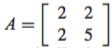
\includegraphics[width=2cm]{figs/2_6_SPD-1} 
%\caption{$f(x) = x^3 + x -1$的图像} 
\end{figure}
就是一个对称正定矩阵,这是因为对任意的$x = [x_1, x_2]^T$,我们有
\begin{figure}
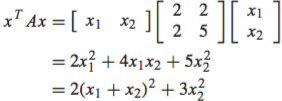
\includegraphics[width=5cm]{figs/2_6_SPD-2} 
%\caption{$f(x) = x^3 + x -1$的图像} 
\end{figure}
$x \neq 0$时结果一定大于$0$。
\end{frame}


\begin{frame}
\frametitle{对称正定矩阵}
而矩阵
\begin{figure}
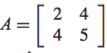
\includegraphics[width=2cm]{figs/2_6_SPD-3} 
%\caption{$f(x) = x^3 + x -1$的图像} 
\end{figure}
不是一个对称正定矩阵,这是因为对任意的$x = [x_1, x_2]^T$,我们有
\begin{figure}
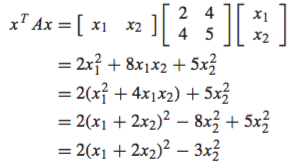
\includegraphics[width=5cm]{figs/2_6_SPD-4} 
%\caption{$f(x) = x^3 + x -1$的图像} 
\end{figure}
如果令$x_1 = -2, x_2 = 1$,则$x^{T}Ax = -1$。
\end{frame}


\begin{frame}
\frametitle{对称正定矩阵的性质}
对称正定矩阵一定是非奇异的,因为如果$A$奇异,则存在$x \neq 0$使得$Ax = 0$,即$x^{T} A x =0$,与$A$正定矛盾。除此之外,对称正定矩阵还有以下性质。

\begin{proposition}
如果$A$是对称矩阵,则$A$是正定的当且仅当$A$的所有特征值是正的。
\end{proposition}

\begin{corollary}
一个对称正定矩阵$A$的行列式是大于$0$的。
\end{corollary}

\begin{proposition}
如果$A$是一个$n\times n$的对称正定矩阵,而$X$是$n \times m$的满秩的矩阵且$n \ge m$,则$X^{T} A X$是一个$m \times m$的对称正定矩阵。
\end{proposition}
\end{frame}


\begin{frame}
\frametitle{对称正定矩阵的性质}
\begin{definition}
如果一个方阵$A$的方子矩阵的对角线上的元素都是$A$的对角线上的元素,则这个方子矩阵称为$A$的主子矩阵。
\end{definition}

\begin{proposition}
对称正定矩阵的任意一个主子矩阵都是对称正定矩阵。
\end{proposition}

\end{frame}


\begin{frame}
\frametitle{对称正定矩阵的Cholesky分解}
\begin{theorem}
如果$A$是一个对称正定矩阵,则一定存在一个$n \times n$的上三角矩阵$R$使得$A = R^T R$
\end{theorem}

\begin{proof}
\ \\
\ \\
\ \\
\ \\
\end{proof}
\begin{remark}
Cholesky分解不是唯一的,因为每一步中对子矩阵左上角的元素$a$开根号可以取正也可以取负。但是,如果限定$R$矩阵的对角线上的元素必须为正数的话,那么Cholesky分解就是唯一的。
\end{remark}
\end{frame}


\begin{frame}
\frametitle{对称正定矩阵的Cholesky分解的算法}
对于这个唯一的Cholesky分解,我们有以下算法
\begin{algorithm}[Cholesky分解算法]\\
{\rm{for}} $k = 0, 1, 2, \ldots, n$ \\
\quad {\rm{if}} $A^k_{11} < 0$ (这里$A^k_{11} < 0$ 表示第$k$步时需要进行分解的子矩阵$A^k$的左上角的元素,$A^k \in \R^{n-k+1 \times n-k+1}$ )\\
\quad \quad 停机,该矩阵不是正定的 \\
\quad $R_{kk} = \sqrt{A^k_{1}}$\\
\quad $u^T = \frac{A^k_{2 : n-k+1}}{R_{kk}}$ ($A^k_{2 : n-k+1}$表示第$k$步时需要进行分解的矩阵$A_k$的第一行除第一个元素之外剩下的元素)\\
\quad $R_{k,k+1:n} = u^T $($R_{k,k+1:n}$表示R的第$k$行从第$k+1$列到第$n$列的元素)\\
\quad $A^{k+1} = A^k_{ 2:n-k+1, 2:n-k+1} - uu^T$(赋值符号右边的$A^k_{ 2:n-k+1, 2:n-k+1}$矩阵$A^k$除第一行第一列之外剩下的部分构成的子矩阵)\\
{\rm{end}}
\end{algorithm}
\end{frame}


\begin{frame}
\frametitle{Cholesky分解举例}
找到以下矩阵的Cholesky分解
\begin{figure}
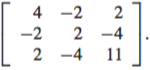
\includegraphics[width=3cm]{figs/2_5_Cholesky-Examp-1} 
%\caption{$f(x) = x^3 + x -1$的图像} 
\end{figure}
首先有$R_{11} = \sqrt{A_{11}} = 2$,进而$R_{1, 2:3} = \frac{A^1_{2 : 3}}{R_{11}}= \frac{[-2,2]}{2} = [-1,1]$,得到
\begin{figure}
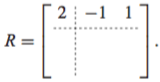
\includegraphics[width=3.5cm]{figs/2_5_Cholesky-Examp-2} 
%\caption{$f(x) = x^3 + x -1$的图像} 
\end{figure}
\end{frame}

\begin{frame}
\frametitle{Cholesky分解举例}
把将$A^1$去掉第一行和第一列之后剩下的子矩阵$A^1_{2:3, 2:3}$减去$uu^T$得到
\begin{figure}
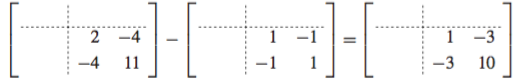
\includegraphics[width=7.5cm]{figs/2_5_Cholesky-Examp-3} 
%\caption{$f(x) = x^3 + x -1$的图像} 
\end{figure}
接下来我们利用$2\times2$正定对称矩阵的Cholesky分解方法对
\begin{figure}
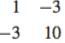
\includegraphics[width=1cm]{figs/2_5_Cholesky-Examp-4} 
%\caption{$f(x) = x^3 + x -1$的图像} 
\end{figure}
进行分解,最终得到
\begin{figure}
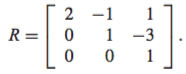
\includegraphics[width=3cm]{figs/2_5_Cholesky-Examp-5} 
%\caption{$f(x) = x^3 + x -1$的图像} 
\end{figure}
\end{frame}


\begin{frame}
\frametitle{利用Cholesky分解的结果解方程组}
用Cholesky分解解方程组的方法与$LU$分解一样,我们有
\begin{align}
Ax = R^TR x = b
\end{align}
等价于求解
\begin{align}
R^T y = b \nonumber \\
R x = y.
\end{align}
\end{frame}

%%%%%%%%%%%%%%%%%%%%%%%%%%%%%%%%%%%%%%%%%%

\section{基本迭代法}

\begin{frame}
\frametitle{迭代法}
我们在解非线性方程时用到了迭代法,基本思想就是把原方程作一个等价变换变成一个求函数不动点,之后不断对迭代函数进行迭代计算,如果得到的是收敛数列则这个收敛数列的极限就是不动点,即原方程的解。

\vspace{0.2cm}

解线性方程组我们也可以利用类似的思想,将方程组化为一个(线性的)多元函数的不动点的问题进行迭代,如果得到的向量序列是收敛的,那么我们就得到了这个(线性的)多元函数的不动点,也就是线性方程组的解。

\vspace{0.2cm}

之前我们所讲的直接法与迭代法最大的区别就在于,直接法在给定的有限步计算之后就一定能得到结果(例如高斯消元是$O(n^3)$的运算),且这个结果是理论上的精确解;而迭代法并不能保证在一定迭代步数之后就得到结果,且得到的结果仍是精确解的一个近似。

\vspace{0.2cm}

虽然迭代法看似不如直接法效果好,但在实际计算中,迭代法对于解线性方程组,尤其是系数矩阵具有特殊结构的线性方程组却是十分有效的方法。

\end{frame}


\begin{frame}
\frametitle{Jacobi迭代}
Jacobi迭代是最简单直接的迭代方法,我们可以用一下这个例子来说明Jacobi迭代法。

\begin{example}
解方程组
\begin{align}
\label{eq: Jacobi_1}
3u + v &= 5 \nonumber \\
u + 2v &= 5.
\end{align}
\end{example}

我们对这个方程组作等价变换,使得第一个方程左边只留下$u$,第二个方程左边只留下$v$得到
\begin{align}
\label{eq: Jacobi_2-1}
u &= \frac{5 - v}{3} \nonumber \\
v &= \frac{5-u}{2}.
\end{align}
\end{frame}


\begin{frame}
\frametitle{Jacobi迭代}
很显然,求方程组\eqref{eq: Jacobi_1}的解等价于求\eqref{eq: Jacobi_2-1}的不动点。如果我们将$(u_0,v_0) = (0,0)$作为初始值进行迭代,将会得到如下计算结果
\begin{figure}
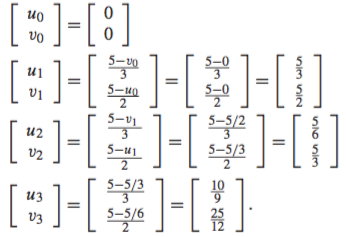
\includegraphics[width=6cm]{figs/2_5_Jacobi-1} 
%\caption{$f(x) = x^3 + x -1$的图像} 
\end{figure}
后续计算结果见Matlab程序Run Jacobi 1。
\end{frame}


\begin{frame}
\frametitle{Jacobi迭代}
如果我们对这个方程组作另一种等价变换,使得第一个方程左边只留下$v$,第二个方程左边只留下$u$得到
\begin{align}
\label{eq: Jacobi_2-2}
u &=5 - 2v \nonumber \\
v &=5 - 3u.
\end{align}
同样将$(u_0,v_0) = (0,0)$作为初始值进行迭代,将会得到如下计算结果
\begin{figure}
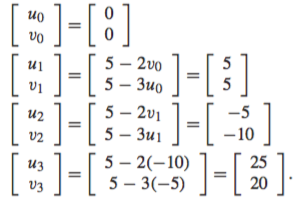
\includegraphics[width=5cm]{figs/2_5_Jacobi-2} 
%\caption{$f(x) = x^3 + x -1$的图像} 
\end{figure}
后续计算结果见Matlab程序Run Jacobi 2(迭代12次达到给定精度)。
\end{frame}


\begin{frame}
\frametitle{Jacobi迭代收敛性的判定}
很明显,第一个迭代产生的向量序列是收敛的,而第二种迭代产生的向量序列是发散的。与解非线性方程的不动点迭代类似,我们需要迭代收敛的判定定理。我们首先有以下定义。

\begin{definition}
一个$n \times n$的矩阵$A = (a_{ij})$,如果对任意$1 \le i \le n$,对角线上的元素$|a_{ii}| > \sum_{i \neq j} |a_{ij}| $,则这个矩阵$A$被称为严格对角占优的。换句话说,对角占优的矩阵在第$i$行中对角线上的元素的绝对值大于这一行中其余所有元素的绝对值的和。
\end{definition}

我们有以下定理:
\begin{theorem}[Jacobi迭代收敛的充分条件]
如果$n \times n$的矩阵$A$是严格对角占优的,那么
\begin{enumerate}
\item $A$是非奇异的(满秩的、可逆的);
\item 对任意的$b$和任意的初始猜测,利用Jacobi迭代解方程组$Ax = b$得到的结果都是收敛的。
\end{enumerate}
\end{theorem}
\end{frame}


\begin{frame}
\frametitle{Jacobi迭代收敛性的判定}
如果我们考虑由\eqref{eq: Jacobi_2-1}和\eqref{eq: Jacobi_2-2}所定义的迭代函数,可以发现这两个函数实际上都是由$Ax = b$等价变换使第$i$个方程左端只剩下第$i$个未知数得到的,只是对于第一个迭代函数
\begin{figure}
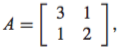
\includegraphics[width=2cm]{figs/2_5_Jacobi-3} 
%\caption{$f(x) = x^3 + x -1$的图像} 
\end{figure}
而对于第二个迭代函数
\begin{figure}
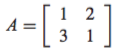
\includegraphics[width=2cm]{figs/2_5_Jacobi-4} 
%\caption{$f(x) = x^3 + x -1$的图像} 
\end{figure}
很明显,对于第一个方程组系数矩阵是严格对角占优的,而对于第二个方程组系数矩阵不是严格对角占优的。\begin{remark}
方程组对角占优是Jacobi迭代收敛的充分条件而非必要条件,虽然第二个方程组所导出的迭代函数产生了发散的向量序列,但这不代表所有不是严格对角占优的矩阵所导出的Jacobi迭代函数都会产生发散的序列。
\end{remark}
\end{frame}

\begin{frame}
\frametitle{Jacobi迭代收敛性的判定}
考虑一下两个矩阵
\begin{figure}
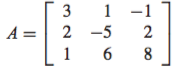
\includegraphics[width=3cm]{figs/2_5_Jacobi-5} 
%\caption{$f(x) = x^3 + x -1$的图像} 
\end{figure}
\begin{figure}
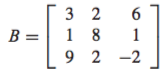
\includegraphics[width=3cm]{figs/2_5_Jacobi-6} 
%\caption{$f(x) = x^3 + x -1$的图像} 
\end{figure}
很明显,矩阵$A$是严格对角占优的,而矩阵$B$不是严格对角占优的。但是如果我们将$B$矩阵的第一行和第三行交换位置,则新的$B$矩阵就变成了严格对角占优的矩阵。
\end{frame}


\begin{frame}
\frametitle{Jacobi迭代的矩阵形式}
Jacobi迭代函数产生的机制就是将$Ax = b$作等价变换,使第$i$个方程左端只剩下第$i$个未知数,这时方程组的右端就是迭代函数。这个过程也可以用矩阵的形式表示出来。

我们令$D$矩阵对角线上的元素与系数矩阵$A$的对角线上的元素相等,其余部分为$0$;$L$矩阵在对角线以下的元素与矩阵$A$对角线以下的元素相等,其余部分为$0$;$U$矩阵在对角线以上的元素与矩阵$A$对角线以上的元素相等,其余部分为$0$。我们有
\begin{equation}
A = L + D + U,
\end{equation}
进而原方程组可以写为
\begin{equation}
Ax = Lx + Dx + Ux = b.
\end{equation}
对这个方程组作等价变换得到
\begin{align}
Lx + Dx + Ux &= b \nonumber \\
                 Dx &= b - (L+U) x \nonumber \\
                    x &= D^{-1} (b - (L+U) x).
\end{align}
\end{frame}


\begin{frame}
\frametitle{Jacobi迭代的算法}
一个对角矩阵$D$的逆也是一个对角矩阵$D^{-1}$,其中$D^{-1}$中对角线上的元素就是$D$的对角矩阵角线上相应位置的元素的倒数,因此求$D^{-1}$的运算量非常小,因此Jacobi迭代的算法如下
\begin{algorithm}[Jacobi迭代算法]\\
设$x^0$为初始猜测\\
{\rm{for}} $k = 0, 1, 2, \ldots$ \\
\quad $x^{k+1} = D^{-1}  (b - (L+U) x^{k})$\\
{\rm{end}}
\end{algorithm}
\end{frame}


\begin{frame}
\frametitle{Jacobi迭代的算法}
例如对于我们讨论的第一个例子,
\begin{figure}
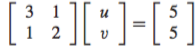
\includegraphics[width=3cm]{figs/2_5_Jacobi-7} 
%\caption{$f(x) = x^3 + x -1$的图像} 
\end{figure}
则Jacobi迭代可以如下算法求得
\begin{figure}
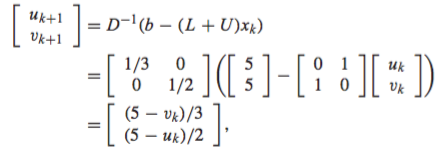
\includegraphics[width=6cm]{figs/2_5_Jacobi-8} 
%\caption{$f(x) = x^3 + x -1$的图像} 
\end{figure}
与我们直接移项得到的形式一致。
\end{frame}


\begin{frame}
\frametitle{Gauss-Seidel迭代和超松弛迭代}
Jacobi迭代的一个变型就是Gauss-Seidel迭代,仍然考虑解方程组
\begin{align}
\label{eq: Jacobi_1}
3u + v &= 5 \nonumber \\
u + 2v &= 5.
\end{align}
对这个方程组使用Gauss-Seidel迭代得到
\begin{figure}
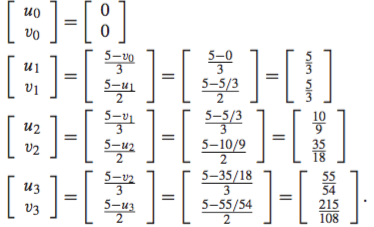
\includegraphics[width=6cm]{figs/2_5_GS-1} 
%\caption{$f(x) = x^3 + x -1$的图像} 
\end{figure}
后续计算结果可见Matlab程序,在这个例子中Gauss-Seidel迭代的收敛速度(6次迭代达到给定精度)比Jacobi迭代要快一些,这在大多数情况下是成立的,但并不是绝对的。
\end{frame}


\begin{frame}
\frametitle{Gauss-Seidel迭代与Jacobi迭代}
Gauss-Seidel迭代和Jacobi迭代形式上非常类似,其的不同之处在于:
\begin{itemize}
\item 在作等价变换使第$i$个方程左端只剩下第$i$个未知数之后,Jacobi迭代直接将右端的函数作为迭代函数,计算时,右端函数中的未知数的值都代为上一步迭代的计算结果;
\item 而Gauss-Seidel迭代中,每当左端的某一个未知量的值有了更新就会马上被代入到右端去进行计算。
\end{itemize}
与Jacobi迭代一样,我们有
\begin{theorem}[Gauss-Seidel迭代收敛的充分条件]
如果$n \times n$的矩阵$A$是严格对角占优的,那么
\begin{enumerate}
\item $A$是非奇异的(满秩的、可逆的);
\item 对任意的$b$和任意的初始猜测,利用Gauss-Seidel迭代解方程组$Ax = b$得到的结果都是收敛的。
\end{enumerate}
\end{theorem}
\end{frame}


\begin{frame}
\frametitle{Gauss-Seidel迭代的矩阵形式}
与Jacobi迭代一样,Gauss-Seidel迭代也可以写为矩阵形式,令原方程组为
\begin{equation}
Ax = Lx + Dx + Ux = b,
\end{equation}
则Gauss-Seidel迭代可以写为
\begin{align}
\label{eq: GS matrix form}
(L+D) x^{k+1} &= b - Ux^{k} \nonumber \\
          x^{k+1} &= (L+D)^{-1} (b - Ux^{k}). 
\end{align}
但是这里要注意一个问题,实际计算中我们是不会用到\eqref{eq: GS matrix form},这是因为求$(L+D)^{-1}$的计算量很大。一般来说,求任意矩阵逆的运算量是$O(n^3)$,相当于作一次高斯消元法的计算量(实际上,计算机求矩阵逆的算法基本都要先作一次高斯消元)。
\end{frame}


\begin{frame}
\frametitle{Gauss-Seidel迭代的算法}
为了避免求矩阵的逆,Gauss-Seidel迭代在实际计算中一般不直接用矩阵相乘,而是一个未知量一个未知量的更新,但形式上我们有
\begin{algorithm}[Gauss-Seidel迭代算法]\\
设$x^0$为初始猜测\\
{\rm{for}} $k = 0, 1, 2, \ldots$ \\
\quad $x^{k+1} = D^{-1}  (b - U x^{k} - L x^{k+1})$\\
{\rm{end}}
\end{algorithm}\\
我们再次强调这个算法实际上是一个式子一个式子进行的,而非直接利用矩阵与向量的乘积。
\end{frame}


\begin{frame}
\frametitle{Gauss-Seidel迭代的算法}
例如对于线性方程组
\begin{figure}
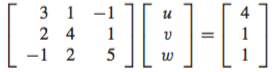
\includegraphics[width=4cm]{figs/2_5_GS-2} 
%\caption{$f(x) = x^3 + x -1$的图像} 
\end{figure}
利用Gauss-Seidel迭代,得到
\begin{figure}
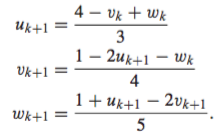
\includegraphics[width=4cm]{figs/2_5_GS-3} 
%\caption{$f(x) = x^3 + x -1$的图像} 
\end{figure}
计算结果可见Matlab程序,由于系数矩阵对角占优,所以最终结果(迭代11次)收敛到$[2,-1,1]^T$。
\end{frame}


\begin{frame}
\frametitle{超松弛迭代(SOR)}
如果我们将Gauss-Seidel迭代的右端项与迭代的上一步结果作一个线性组合,就得到了松弛迭代,例如对于上面考虑的方程组,我们得到
\begin{figure}
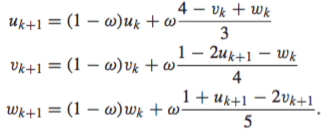
\includegraphics[width=6cm]{figs/2_5_SOR-1} 
%\caption{$f(x) = x^3 + x -1$的图像} 
\end{figure}
这里$\omega$称为松弛系数,如果这个松弛系数大于1,则这个迭代称为超松弛迭代。使用超松弛迭代的原因是我们希望在保持迭代为不动点迭代的前提下,利用Gauss-Seidel迭代收敛速度快的优势加速迭代的收敛。例如在上面的例子中令$\omega = 1.25$,我么可以利用Matlab来观察计算过程(迭代7次就达到要求的精度)。
\end{frame}


\begin{frame}
\frametitle{(超)松弛迭代(SOR)的矩阵形式及算法}
对于(超)松弛迭代,我们实际上是在原方程组两边同时乘以了一个系数$\omega$,得到
\begin{align}
(\omega L + \omega D + \omega U) x & = \omega b  \nonumber \\      
(\omega L + D) x &= \omega b - \omega U x + (1 - \omega)Dx \nonumber \\
                                                         x & =  (\omega L + D)^{-1} [(1- \omega)Dx - \omega Ux] + \omega (D + \omega L)^{-1} b.                          
\end{align}
我们进而得到SOR的算法
\begin{algorithm}[SOR迭代算法]\\
设$x^0$为初始猜测\\
{\rm{for}} $k = 0, 1, 2, \ldots$ \\
\quad $x^{k+1} = (\omega L + D)^{-1} [(1- \omega)Dx^{k} - \omega Ux^{k}] + \omega (D + \omega L)^{-1} b$\\
{\rm{end}}
\end{algorithm}\\
\end{frame}


\begin{frame}
\frametitle{三种算法的比较}
如果我们利用三种迭代解线性方程组
\begin{figure}
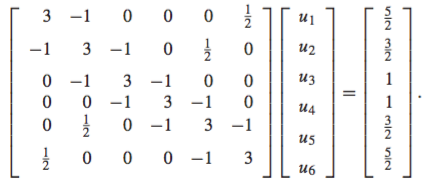
\includegraphics[width=6.5cm]{figs/2_5_SOR-2} 
%\caption{$f(x) = x^3 + x -1$的图像} 
\end{figure}
迭代六步之后我们得到的结果见下表
\begin{figure}
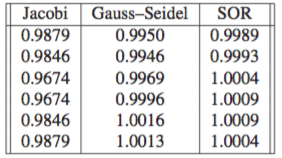
\includegraphics[width=4.5cm]{figs/2_5_SOR-3} 
%\caption{$f(x) = x^3 + x -1$的图像} 
\end{figure}
而真实解为$x = [1,1,1,1,1,1]^T$
\end{frame}

\begin{frame}
\frametitle{三种算法的比较}
在这个例子中,SOR迭代相对较好。但是我们再次强调,每一种算法都不是一定比其它算法好,甚至对于同一个问题会出现有些算法收敛而其它算法发散的情况,因此要根据实际情况进行判断算法的优劣性。对于SOR算法中$\omega$的取值也没有一个对任何问题都有效的判定标准,只有一些特殊问题可以理论上得到最优的$\omega$取值。
\end{frame}


\begin{frame}
\frametitle{使用迭代法的必要性}
高斯消元给出了有限步计算得到精确解的算法,而迭代法的收敛性和迭代步数都是不确定,那么为什么我们还要探讨迭代法呢?

\vspace{0.2cm}

最重要的原因事实上是计算量。牛顿迭代,包括$LU$分解的计算量都是$O(n^3)$,而迭代法中,每一步迭代(相当于作几次矩阵与向量相乘)的计算量最多是$O(n^2)$,如果$n$很大,而达到足够精度的迭代步数远小于$n$的话,那么一次迭代法的计算量就比高斯消元要小。特别是在以下两种情况之下迭代法都是好的选择。
\end{frame}


\begin{frame}
\frametitle{$A$与$b$的微小变化}
如果我们需要解一系列$Ax = b$的问题,而$A$与$b$都在不断变化,但变化量很小,那么这时候迭代法就比消元试用了,因为上一次利用迭代法得到的计算结果就可以作为下一次迭代法的初值。例如解之前的方程组
\begin{figure}
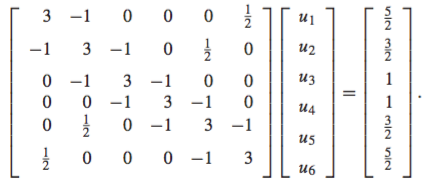
\includegraphics[width=7cm]{figs/2_5_SOR-2} 
%\caption{$f(x) = x^3 + x -1$的图像} 
\end{figure}
如果$b$从$b = [2.5, 1.5, 1, 1, 1.5, 2.5]^T$变为$b = [2.2, 1.6, 0.9, 1.3, 1.4, 2.45]^T$,可以验证这个方程组的解从$x =[1,1,1,1,1,1]^T$变为$x = [0.9, 1, 1, 1, 1, 1]^T$。
\end{frame}


\begin{frame}
\frametitle{$A$与$b$的微小变化}
如果我们以上一次迭代的第六步结果作为迭代初值,则利用Gauss-Seidel迭代再迭代两步后的结果是
\begin{figure}
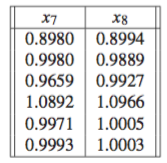
\includegraphics[width=3.5cm]{figs/2_5_SOR-4} 
%\caption{$f(x) = x^3 + x -1$的图像} 
\end{figure}
这种方法称为润色,在实际计算中有很多的应用,尤其是当数据不断更新的情况。
\end{frame}


\begin{frame}
\frametitle{稀疏矩阵的处理}
迭代法在矩阵为稀疏矩阵的情况下有更大的作用。如果一个$n \times n$的矩阵非零元素的个数为$O(n)$的话,则这个矩阵称为稀疏矩阵;而如果一个$n \times n$的矩阵非零元素的个数为$O(n^2)$的话,则这个矩阵称为稠密矩阵。

\vspace{0.2cm}

稀疏矩阵虽然非零元素比较少,但是如果对稀疏矩阵作$PA = LU$分解的话,很容易出现填充(fill-in)现象,也就是说一个稀疏矩阵的$PA = LU$分解出来的$L$与$U$往往不再是稀疏的,这样即便得到了$PA = LU$分解也需要$O(n^2)$的运算才能得到方程的解。而如果对于稀疏矩阵作迭代的话每次计算量是$O(n)$。这样如果迭代收敛速度比较快的话,可以省下很多的计算量。
\end{frame}


\begin{frame}
\frametitle{稀疏矩阵的处理}
例如我们解$100,000$阶的类似于上面的例子中的方程组,则稀疏矩阵的形式大致是(例如$n = 12$)
\begin{figure}
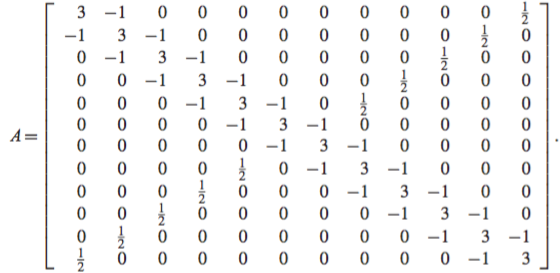
\includegraphics[width=7.5cm]{figs/2_5_SOR-5} 
%\caption{$f(x) = x^3 + x -1$的图像} 
\end{figure}
而右端项为$b = [2.5, 1.5, \ldots, 1.5, 1.0, 1.0, 1.5, \ldots, 1.5, 2.5]^T$。
\end{frame}


\begin{frame}
\frametitle{稀疏矩阵的处理}
如果我们把这个矩阵的所有元素,包括零元素储存下来,则这个矩阵有$n^2 = 10^{10}$个元素,如果没有元素用IEEE双精度浮点数储存,每个数的储存需要$8$个字节,则一共需要$8 \times 10^{10}$字节,这大约是80个G的储存量。一般台式机的内存是无法存下这个矩阵的。

\vspace{0.2cm}

除此之外,对这个矩阵作$PA = LU$分解需要$n^3 \approx 10^{15}$次运算,如果你的CPU是1 GHz(大约$10^9$个周期每秒),则浮点运算速度的上界大约为$10^8$次计算每秒。那么这个$PA = LU$分解需要$10^7$秒,这大概等于4个月的时间。

\vspace{0.2cm}

而对于这个方程组作一次迭代运算,其运算量大概是$800,000 \approx 10^6$次,即便我们作$100$步的迭代,我们也只需要1秒的时间。而对于上面我们考虑的问题,实际上迭代法只需要$27$步就可以从初始猜测$x^0 = [0,0, \ldots, 0, 0]$收敛到真实解$[1,1,\ldots,1,1]$。计算程序和结果见Matlab程序,需要注意我们使用了Matlab的spdiags函数用以生成稀疏矩阵,在Matlab中,稀疏矩阵的存储量大约只有稀疏矩阵非零元素的个数,即$O(n)$。


\end{frame}


%%%%%%%%%%%%%%%%%%%%%%%%%%%%%%%%%%%%%%%%%%



\section{求解非线性方程组}

\begin{frame}
\frametitle{求解非线性方程组}
求解线性方程组有许多重要的应用,其中之一是求解非线性方程组。我们上一讲中讨论了如何解非线性方程,我们现在讨论如何求解非线性方程组。我们以一个由三个方程组成的三元方程组为例来探讨这个问题。例如求解$F(u,v, w) = (f_1, f_2, f_3)^T = 0$,或$F(x) = 0$, $x = [u,v,w]^T$,即
\begin{align}
\label{eq: nonlinear system 3 variable general}
f_1(u,v,w) &= 0 \nonumber \\
f_2(u,v,w) &= 0 \nonumber \\
f_3(u,v,w) &= 0.
\end{align}

我们首先定义$F(x)$的Jacobi矩阵为
\begin{figure}
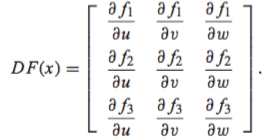
\includegraphics[width=4cm]{figs/2_6_Nonlinear-General-1} 
%\caption{$f(x) = x^3 + x -1$的图像} 
\end{figure}
Jacobi矩阵实际上是一元函数导数在多元方程组中的推广。
\end{frame}


\begin{frame}
\frametitle{求解非线性方程组的牛顿迭代}
求解非线性方程组的基本方法就是牛顿迭代,也就是说,我们要把一元方程的牛顿迭代
\begin{equation}
x^{k+1} = x^{k}  - \frac{f(x^k)}{f'(x^{k+1})}
\end{equation}
推广到多元方程组中去。
我们首先利用多元方程组在$x_0 = [u_0, v_0, w_0]^T$处的Taylor展开,得到
\begin{equation}
F(x) = F(x_0) + DF(x_0) (x-x_0) + O(\|x-x_0\|^2).
\end{equation}
这里$DF(x_0) (x-x_0)$表示矩阵$DF(x_0)$与向量$x-x_0$相乘
\end{frame}


\begin{frame}
\frametitle{求解非线性方程组的牛顿迭代}
例如,如果$F(u,v) = (e^{u+v}, \sin u)$,则在$x_0 = (0,0)$附近有
\begin{figure}
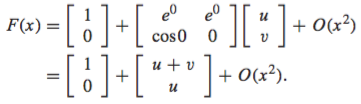
\includegraphics[width=7cm]{figs/2_6_Nonlinear-General-2} 
%\caption{$f(x) = x^3 + x -1$的图像} 
\end{figure}
\end{frame}


\begin{frame}
\frametitle{求解非线性方程组的牛顿迭代}
非线性方程组的牛顿迭代构造的基本思想与非线性方程的一样,都是忽略高阶项$O(x^2)$。若令$x = r$是非线性方程组的根,则
\begin{equation}
0 = F(r) \approx F(x_0) + DF(x_0) (r-x_0),
\end{equation}
移项得
\begin{equation}
x_0-DF(x_0)^{-1} F(x_0) \approx r.
\end{equation}
具体的算法是

\begin{algorithm}[非线性方程组的牛顿代算法]\\
设$x^0$为初始猜测\\
{\rm{for}} $k = 0, 1, 2, \ldots$ \\
\quad $x^{k+1} = x^{k} -DF(x^{k})^{-1} F(x^{k})$\\
{\rm{end}}
\end{algorithm}\\
\end{frame}


\begin{frame}
\frametitle{求解非线性方程组的牛顿迭代}
由于求矩阵的逆计算量大约是高斯消元的3倍,因此在实际计算中我们并不求$DF(x^{k})^{-1}$,而是求解关于$s$的方程组
\begin{equation}
DF(x^{k}) s = - F(x^{k}),
\end{equation}
之后再计算
\begin{equation}
x^{k+1} = x^k + s.
\end{equation}

\begin{example}
求解方程组
\begin{align}
v - u^3 = 0 \nonumber \\
u^2 + v^2 -1 = 0
\end{align}
\end{example}
\end{frame}


\begin{frame}
\frametitle{求解非线性方程组的牛顿迭代举例}
以上方程组的解可以由下图大致表示出来
\begin{figure}
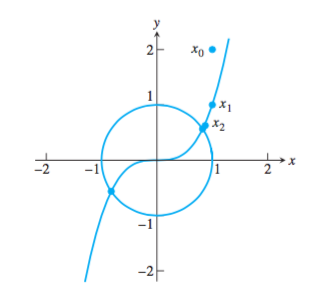
\includegraphics[width=5cm]{figs/2_6_Nonlinear-Examp-1-1} 
\caption{$f_1(u,v) = v - u^3 =0$和$f_2(u,v) = u^2 + v^2 -1=0$的图像} 
\end{figure}
\end{frame}


\begin{frame}
\frametitle{求解非线性方程组的牛顿迭代举例}
为了精确求解原线性方程组,我们首先找到它的Jacobi矩阵
\begin{figure}
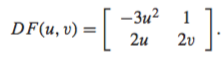
\includegraphics[width=4cm]{figs/2_6_Nonlinear-Examp-1-2} 
%\caption{$f_1(u,v) = v - u^3 =0$和$f_2(u,v) = u^2 + v^2 -1=0$的图像} 
\end{figure}
如果我们以$x_0 = [1,2]^T$为初值,则第一步中,我们首先要解
\begin{figure}
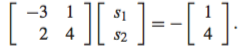
\includegraphics[width=4cm]{figs/2_6_Nonlinear-Examp-1-3} 
%\caption{$f_1(u,v) = v - u^3 =0$和$f_2(u,v) = u^2 + v^2 -1=0$的图像} 
\end{figure}
得到$s = [0,-1]^T$,进而$x^{1} = x^0 + s = [1,1]^T$.
\end{frame}


\begin{frame}
\frametitle{求解非线性方程组的牛顿迭代举例}
第二步我们更新Jacobi矩阵和$F(x)$的值,得到
\begin{figure}
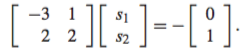
\includegraphics[width=4cm]{figs/2_6_Nonlinear-Examp-1-4} 
%\caption{$f_1(u,v) = v - u^3 =0$和$f_2(u,v) = u^2 + v^2 -1=0$的图像} 
\end{figure}
计算得$s = [-\frac{1}{8},-\frac{3}{8}]^T$,进而$x^{2} = x^1 + s = [\frac{7}{8},\frac{5}{8}]^T$.
后续计算见下表
\begin{figure}
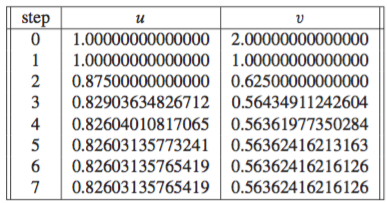
\includegraphics[width=6cm]{figs/2_6_Nonlinear-Examp-1-5} 
%\caption{$f_1(u,v) = v - u^3 =0$和$f_2(u,v) = u^2 + v^2 -1=0$的图像} 
\end{figure}
如果我们从$[-1,-2]^T$开始迭代就会收敛到$y-$轴左边的根,具体计算结果见Matlab程序。
\end{frame}


\begin{frame}
\frametitle{求解非线性方程组的牛顿迭代举例}
\begin{example}
求解方程组
\begin{align}
f_1(u,v) = 6u^3 + uv - 3v^3 - 4= 0 \nonumber \\
f_2(u,v) = u^2 - 18uv^2 + 16v^3 + 1 = 0
\end{align}
\end{example}
首先求Jacobi矩阵
\begin{figure}
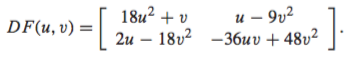
\includegraphics[width=6.5cm]{figs/2_6_Nonlinear-Examp-1-6} 
%\caption{$f_1(u,v) = v - u^3 =0$和$f_2(u,v) = u^2 + v^2 -1=0$的图像} 
\end{figure}
\end{frame}


\begin{frame}
\frametitle{求解非线性方程组的牛顿迭代举例}
从初始猜测$[u_0, v_0] = [2,2]^T$开始得到如下结果
\begin{figure}
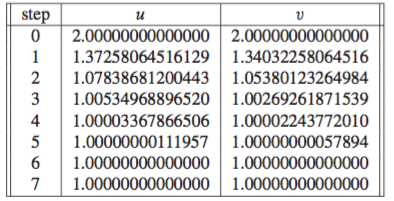
\includegraphics[width=7cm]{figs/2_6_Nonlinear-Examp-1-7} 
%\caption{$f_1(u,v) = v - u^3 =0$和$f_2(u,v) = u^2 + v^2 -1=0$的图像} 
\end{figure}
从其它点上迭代得到的根见Matlab程序。
\end{frame}

%%%%%%%%%%%%%%%%%%%%%%%%%%%%%%%%%%%%%%%%%%

\begin{frame}
\frametitle{课后阅读}
[NA] 第2章 2.6.1,2.6.2,2.5.1, 2.5.2, 2.5.4,2.7.1


\end{frame}

\end{document}

